\section{Process and Results}

\subsection{Capital Asset Pricing Model}
To determine the CAPM for each asset, we must first calculate the Risk-Free Rate (\(R_f\)), Expected Market Return (\(R_m\)), Beta (\(\beta\)) for each asset. Below lays out the steps

1. Risk-Free Rate (\(R_f\))

The risk-free rate is typically the return on government bonds, such as U.S. Treasury bills. We decided to use the average risk-free rate over our analysis period for CBOE Interest Rate 10 Year T No \cite{YahooFinanceTNX}

2. Expected Market Return (\(R_m\))

To measure the expected market return, we decided to align our focus to the cryptocurrency market. The expected market return is the average return of a broad cryptocurrency market index, and we used the Bitwise 10 Crypto Index Fund (BITW) \cite{bitw}.

3. Beta Calculation (\(\beta\))

Beta measures the volatility of an asset relative to the market. 

\begin{itemize}
    \item Obtained historical daily prices for each asset and the chosen market index.
    \item Computed the daily returns for each asset and the market index.
    \item Performed a linear regression with the asset returns as the dependent variable and the market index returns as the independent variable. The slope of the regression line is the beta.
\end{itemize}

4. Market Risk Premium (\(R_m - R_f\))

The market risk premium is the difference between the expected market return and the risk-free rate.

Combining each component into the CAPM Model, we obtained the following results.

\begin{table}[h]
\centering
\begin{tabular}{|c|c|c|c|}
\hline
\textbf{Asset} & \textbf{Beta} & \textbf{Market Risk Premium} & \textbf{Expected Return (CAPM)} \\
\hline
AAPL & 0.1489 & -0.0346 & 0.0294 \\
MSFT & 0.1469 & -0.0346 & 0.0295 \\
AMZN & 0.2194 & -0.0346 & 0.0270 \\
GOOGL & 0.1653 & -0.0346 & 0.0289 \\
TSLA & 0.2734 & -0.0346 & 0.0251 \\
SPY & 0.1084 & -0.0346 & 0.0308 \\
DJI & 0.0089 & -0.0346 & 0.0343 \\
AGG & 0.0115 & -0.0346 & 0.0342 \\
VNQ & 0.0884 & -0.0346 & 0.0315 \\
GLD & 0.0195 & -0.0346 & 0.0339 \\
USO & 0.0408 & -0.0346 & 0.0332 \\
SLV & 0.0671 & -0.0346 & 0.0323 \\
PSP & 0.1596 & -0.0346 & 0.0291 \\
BTC-USD & 0.4680 & -0.0346 & 0.0184 \\
ETH-USD & 0.5448 & -0.0346 & 0.0157 \\
SOL-USD & 0.7253 & -0.0346 & 0.0095 \\
BNB-USD & 0.3944 & -0.0346 & 0.0209 \\
XRP-USD & 0.5699 & -0.0346 & 0.0149 \\
TON-USD & 0.4154 & -0.0346 & 0.0202 \\
DOGE-USD & 0.4995 & -0.0346 & 0.0173 \\
ADA-USD & 0.5541 & -0.0346 & 0.0154 \\
SHIB-USD & 0.5231 & -0.0346 & 0.0165 \\
AVAX-USD & 0.6062 & -0.0346 & 0.0136 \\
\hline
\end{tabular}
\caption{CAPM Estimates for Various Assets}
\label{tab:capm}
\end{table}


More information can be found in appendix, please refer to \ref{appendix:capm_details}.

\begin{figure}
    \centering
    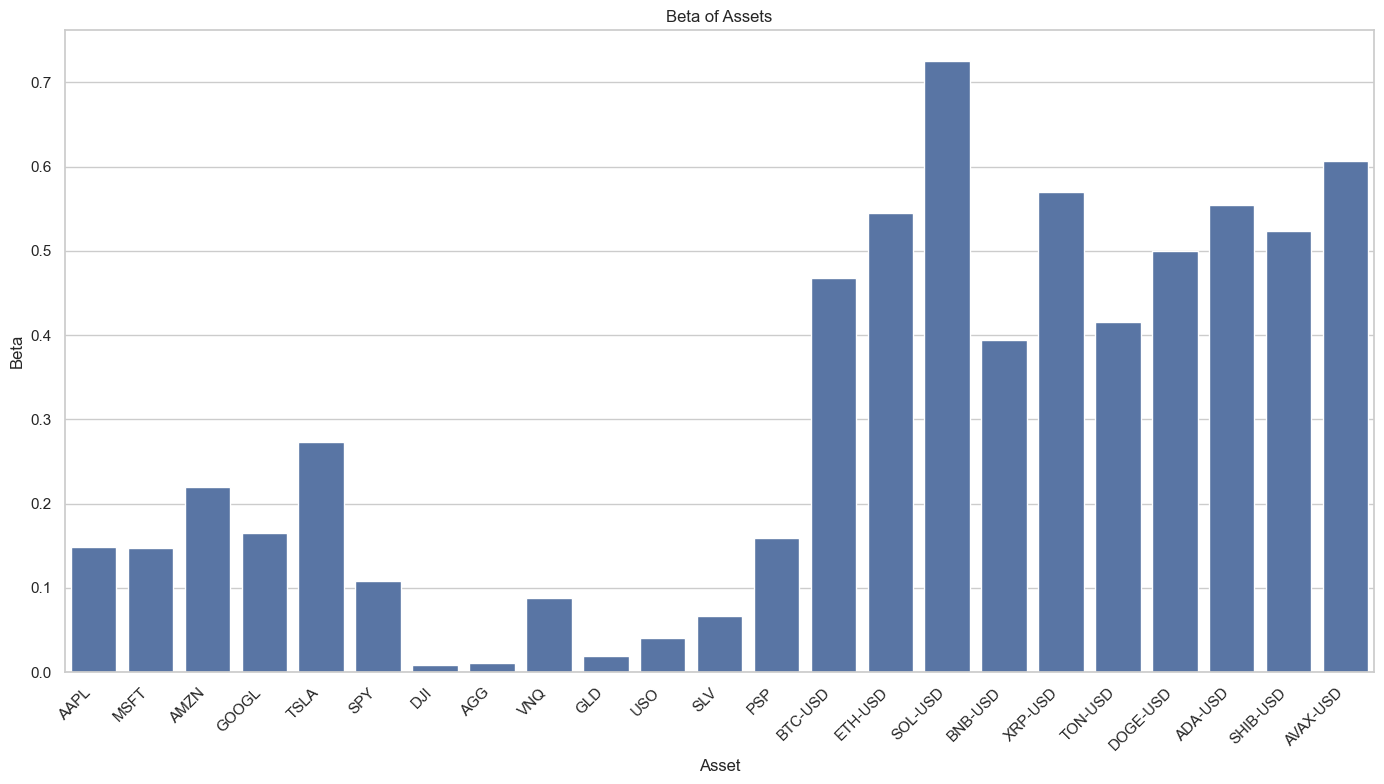
\includegraphics[width=\textwidth]{./code/risk-and-return-analysis/capm/beta_assets.png}
    \caption{Beta of Assets Relative to BITW}
    \label{fig:beta}
\end{figure}

\begin{figure}
    \centering
    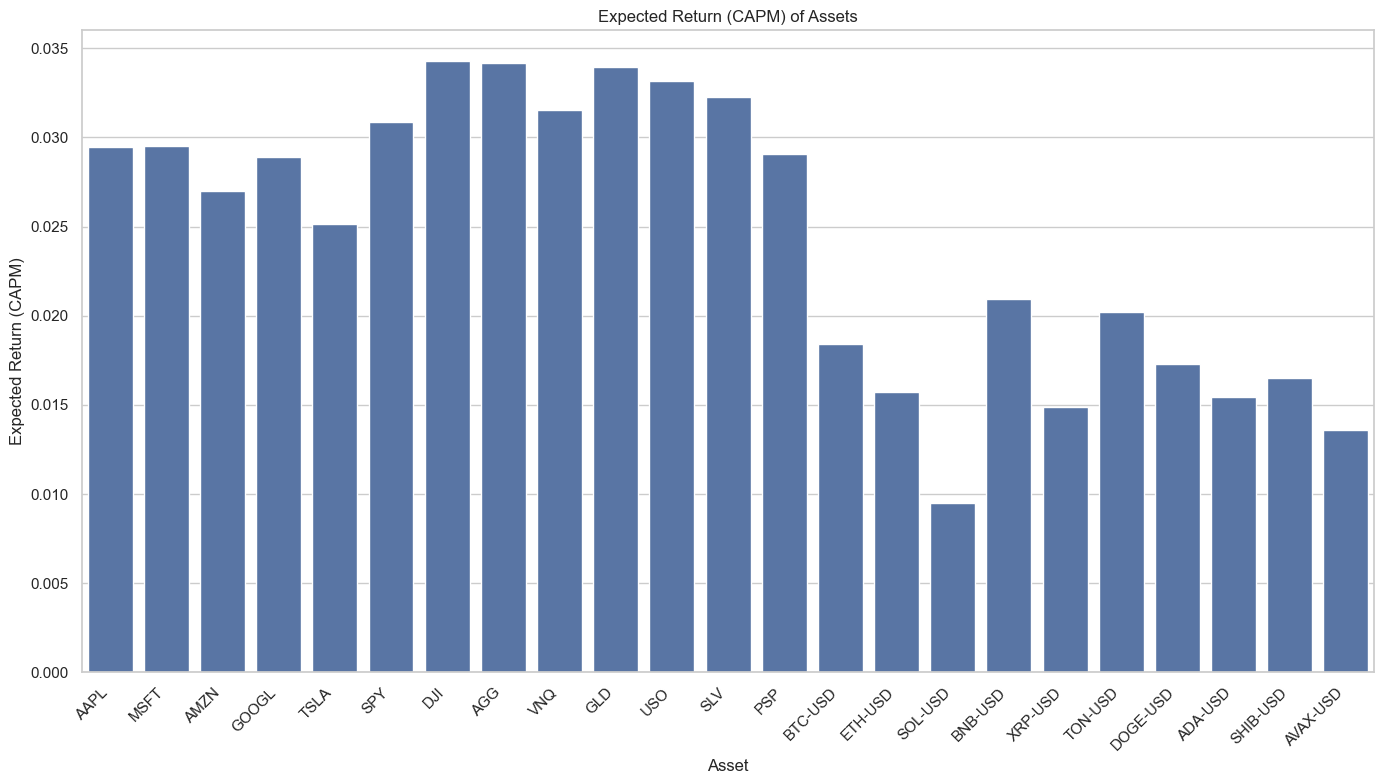
\includegraphics[width=\textwidth]{./code/risk-and-return-analysis/capm/exp_return_assets.png}
    \caption{Expected Return of Assets Relative to BITW}
    \label{fig:exp_return}
\end{figure}


\subsection{GARCH Model}

To investigate the time-varying volatility of different financial assets via the GAR Model, we first calculated the daily returns of each asset. Next, we specified and fitted a GARCH(1,1) model to the return data for each asset. This model choice is common in finance for capturing volatility clustering. After fitting the models, we evaluated their performance using various criteria. This included examining summary statistics, such as the Akaike Information Criterion (AIC) and Bayesian Information Criterion (BIC), to assess model fit and complexity. Additionally, we analyzed residuals to ensure they exhibited characteristics of white noise and conducted stationarity tests to validate model assumptions. Finally, we performed out-of-sample forecasting to assess the model's predictive ability.

\begin{figure}
    \centering
    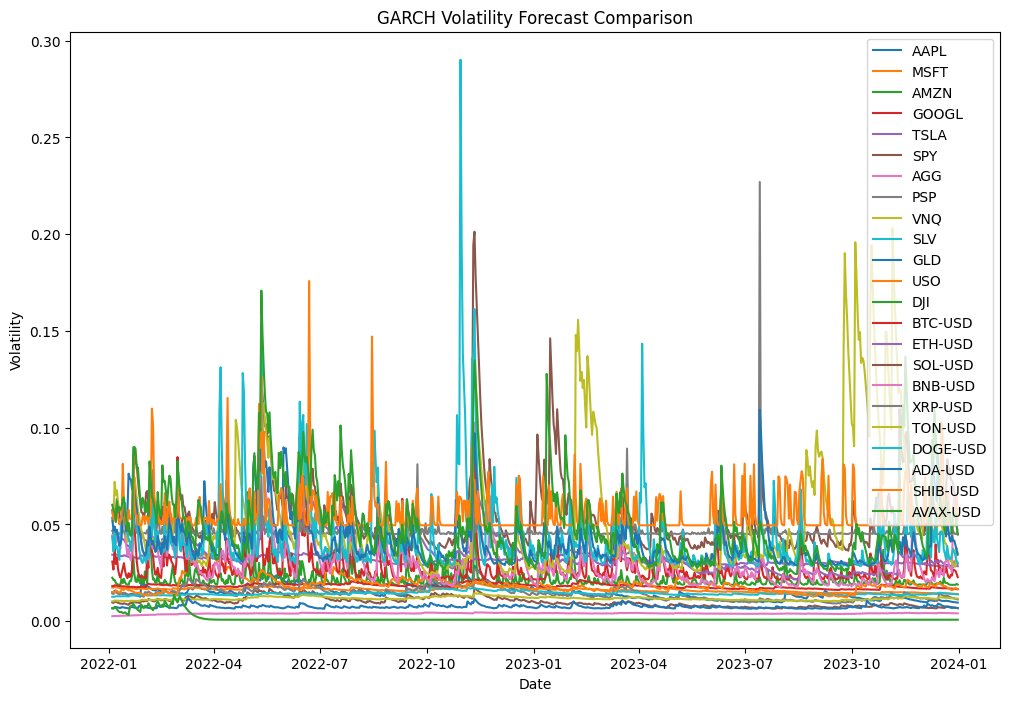
\includegraphics[width=\textwidth]{code/volatility-analysis/garch-with-mulit-assets/garch_forecast.png}
    \caption{GARCH Volatility Forecast}
    \label{fig:exp_return}
\end{figure}

\begin{figure}
    \centering
    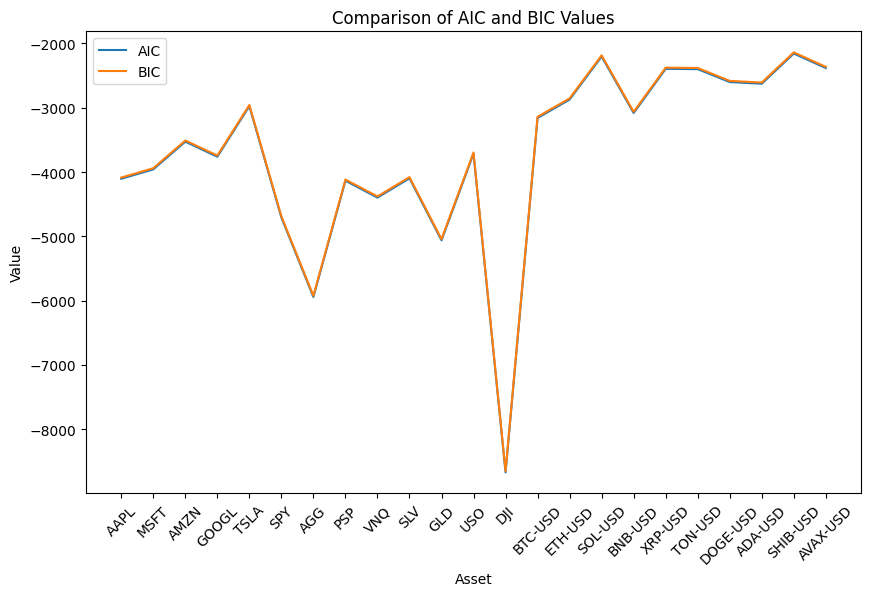
\includegraphics[width=\textwidth]{code/volatility-analysis/garch-with-mulit-assets/aic_bic.png}
    \caption{Comparison between AIC and BIC Values}
    \label{fig:exp_return}
\end{figure}

\begin{figure}
    \centering
    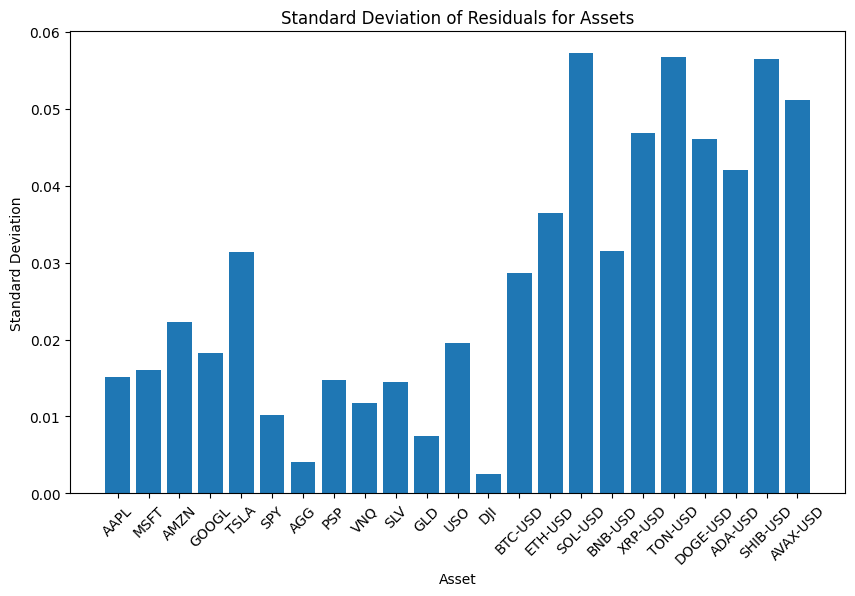
\includegraphics[width=\textwidth]{code/volatility-analysis/garch-with-mulit-assets/standard_deviation.png}
    \caption{Standard Deviation of Residuals}
    \label{fig:exp_return}
\end{figure}



\subsection{Valuation}

For cryptocurrencies:
\[
\text{Intrinsic Value} = \frac{P \times Q}{V}
\]

Results

\begin{figure}
    \centering
    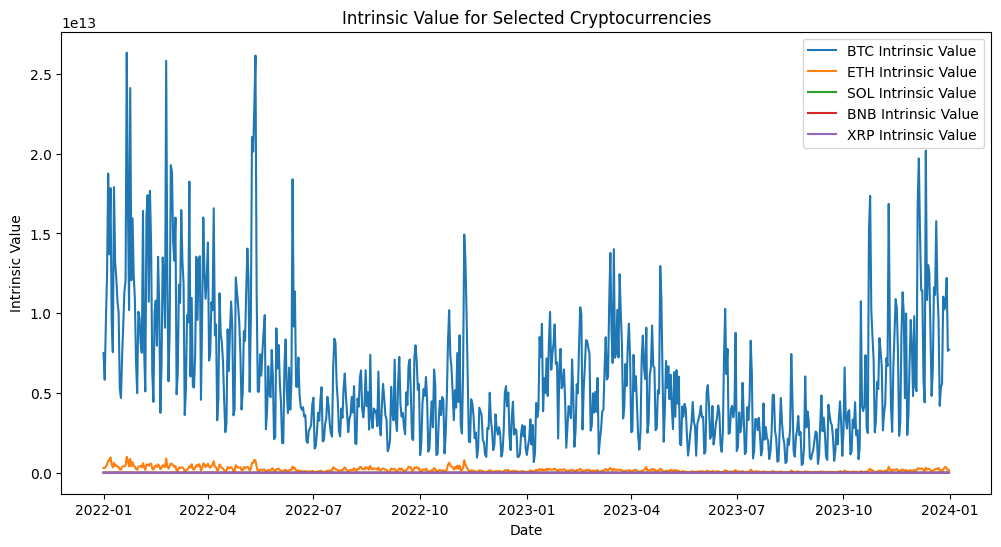
\includegraphics[width=0.8\textwidth]{./code/valuation-techniques/intrinsic_value.png}
    \caption{Intrinsic Value }
    \label{fig:beta}
\end{figure}

\begin{figure}
    \centering
    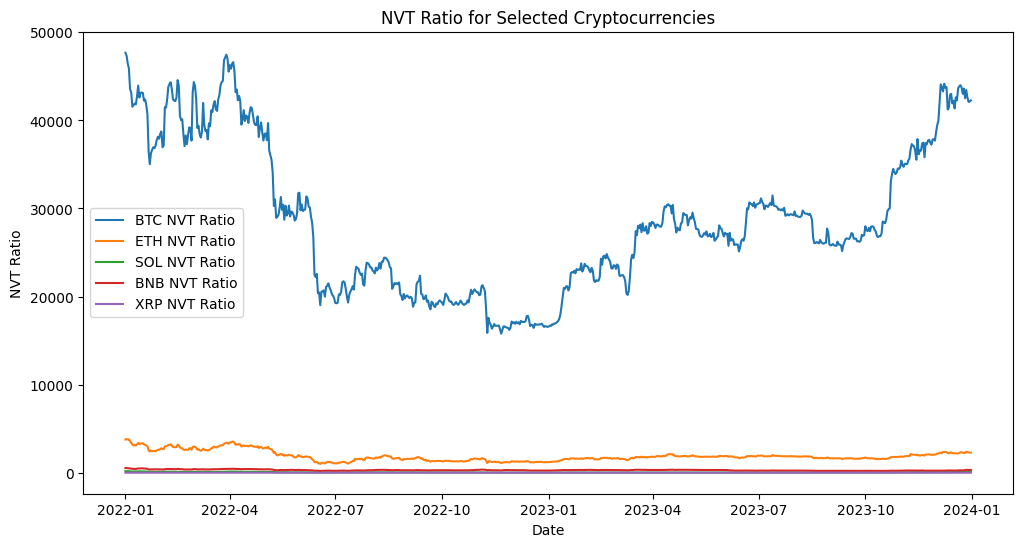
\includegraphics[width=0.8\textwidth]{./code/valuation-techniques/nvt_ratio.png}
    \caption{Network Value to Transactions Ratios}
    \label{fig:beta}
\end{figure}

We have to make some assumptions or gather data for $V$ (velocity), $P$ (price level), and $Q$ (transaction volume).